\chapter{De rekreflex en de zenuwboodschap}\label{ch:g12:stretch-reflex}

Een arts tikt met een klein rubberen hamertje op de \omterm{def:g10:muscles-and-joints:muscle}{pees} vlak onder je
knieschijf, en je voet schopt naar voren voordat je iets hebt gevoeld.
Dertig milliseconden liggen er tussen de tik en de schop: te weinig voor
de hersenen, te weinig zelfs voor een beslissing. Het signaal ging van de
spier naar het ruggenmerg en terug --- een kring van twee \omterm{def:g12:stretch-reflex:neuron}{neuronen} en één
verbinding daartussen --- en diezelfde kring is wat je in stilte
rechtop houdt, elke seconde dat je staat. Dit hoofdstuk gebruikt hem om
het \omterm{def:g12:stretch-reflex:neuron}{neuron} in te leiden, het elektrische signaal dat het draagt, en de
chemische overgang waar het ene \omterm{def:g12:stretch-reflex:neuron}{neuron} tegen het volgende spreekt.

\section{De reflexboog}

\begin{definition}[Reflex]\label{def:g12:stretch-reflex:reflex}
Een \emph{reflex}\index{reflex} is een onwillekeurige, snelle en steeds
gelijke reactie van een uitvoerder (een spier of een klier) op een
prikkel, voortgebracht door een vaste kring \omterm{def:g12:stretch-reflex:neuron}{neuronen}, de
\emph{reflexboog}\index{reflexboog}, die door het ruggenmerg of de
hersenstam loopt zonder dat de hersenen nodig zijn. De
\emph{rekreflex}\index{rekreflex} is de eenvoudigste: een spier plotseling
uitrekken laat diezelfde spier samentrekken.
\end{definition}

\begin{proposition}[De kring van de rekreflex]\label{prop:g12:stretch-reflex:arc}
Vijf onderdelen, op volgorde:
\begin{enumerate}
  \item de \emph{ontvanger}: de \emph{spierspoeltjes}, kleine
        zintuigorgaantjes die tussen de \omterm{def:g10:muscles-and-joints:muscle}{spiervezels} liggen, die worden
        uitgerekt wanneer de spier dat wordt en daarop met signalen
        antwoorden;
  \item het \emph{sensorische \omterm{def:g12:stretch-reflex:neuron}{neuron}}, waarvan de vezel van het spoeltje
        naar het ruggenmerg loopt en er via de achterwortel binnenkomt;
        zijn cellichaam zit in een knoop naast het merg;
  \item het \emph{schakelcentrum}: de grijze stof van het ruggenmerg,
        waar de sensorische vezel rechtstreeks --- door één enkele \omterm{def:g12:stretch-reflex:synapse}{synaps}
        --- met het motorische \omterm{def:g12:stretch-reflex:neuron}{neuron} van diezelfde spier is verbonden
        en, via een tussenneuron, de motorische \omterm{def:g12:stretch-reflex:neuron}{neuronen} van de
        tegenwerkende spier remt;
  \item het \emph{motorische \omterm{def:g12:stretch-reflex:neuron}{neuron}}, waarvan de vezel via de voorwortel
        vertrekt en naar de spier loopt;
  \item de \emph{uitvoerder}: de \omterm{def:g10:muscles-and-joints:muscle}{spiervezels}, die samentrekken.
\end{enumerate}
Een tik op de kniepees rekt de dijspier uit; haar spoeltjes vuren; de
motorische \omterm{def:g12:stretch-reflex:neuron}{neuronen} van die spier vuren; zij trekt samen en het been
strekt, terwijl de kniebuigers te horen krijgen dat zij moeten ontspannen.
\end{proposition}
\begin{proof}[Bewijsmateriaal]
De achterwortel doorsnijden heft de \omterm{def:g12:stretch-reflex:reflex}{reflex} op terwijl de spier nog altijd
tot samentrekken kan worden gebracht door de voorwortel te prikkelen; de
voorwortel doorsnijden heft hem op terwijl de sensorische vezels nog
altijd signalen dragen wanneer de spier wordt uitgerekt: de boog heeft een
sensorische ingang en een motorische uitgang. De \omterm{def:g12:stretch-reflex:reflex}{reflex} blijft bestaan bij
een dier waarvan het ruggenmerg van de hersenen is afgesneden: de hersenen
zijn niet nodig. Opnames van losse vezels laten zien dat de signalen van
het spoeltje binnen een milliseconde na de rek beginnen, en dat het
motorische \omterm{def:g12:stretch-reflex:neuron}{neuron} ongeveer een milliseconde na de aankomst van het
sensorische signaal vuurt --- de vertraging van één \omterm{def:g12:stretch-reflex:synapse}{synaps}.
\end{proof}

\begin{omfigure}
\begin{tikzpicture}[font=\small, >=Stealth, line cap=round]
  % spinal cord section (simplified): outer white, inner grey H
  \draw[thick, fill=omDef!6] (0,0) ellipse (2.2 and 1.5);
  \draw[thick, fill=gray!25] (-0.9,-1.0) -- (-0.9,0.3) .. controls (-0.9,0.9) .. (-0.5,1.0) -- (-0.3,0.4) -- (0.3,0.4) -- (0.5,1.0) .. controls (0.9,0.9) .. (0.9,0.3) -- (0.9,-1.0) .. controls (0.6,-1.1) .. (0.3,-0.5) -- (-0.3,-0.5) .. controls (-0.6,-1.1) .. (-0.9,-1.0) -- cycle;
  \node[font=\scriptsize] at (0,-1.25) {grijze stof};
  \node[anchor=south, font=\scriptsize] at (0,1.6) {ruggenmerg (doorsnede)};
  % sensory neuron: from spindle (right, muscle) to dorsal root (top right) into grey matter
  \draw[thick, omDef] (5.4,1.2) -- (3.2,1.2) -- (2.4,1.1);
  \draw[thick, omDef] (2.4,1.1) .. controls (1.4,0.9) .. (0.55,0.5);
  \fill[omDef] (2.7,1.2) circle (3pt); \node[font=\scriptsize, omDef, anchor=south] at (2.7,1.35) {cellichaam};
  \node[font=\scriptsize, omDef, anchor=south] at (4.4,1.3) {sensorisch neuron};
  % motor neuron: cell body in ventral grey, axon out ventral root to muscle
  \fill[omThm] (0.55,-0.7) circle (4pt);
  \draw[thick, omThm] (0.55,-0.7) .. controls (1.6,-1.2) .. (2.6,-1.3) -- (5.4,-1.3);
  \node[font=\scriptsize, omThm, anchor=north] at (4.2,-1.4) {motorisch neuron};
  % synapse mark
  \fill[omProp] (0.55,0.5) circle (2pt); \draw[omProp, thick] (0.55,0.45) -- (0.55,-0.6);
  \node[font=\scriptsize, omProp, anchor=west] at (1.0,-0.15) {synaps};
  % interneuron to antagonist
  \fill[omMeth!70!black] (-0.5,-0.2) circle (3pt);
  \draw[thick, omMeth!70!black] (0.5,0.5) .. controls (0.0,0.4) .. (-0.5,-0.2);
  \draw[thick, omMeth!70!black, dashed] (-0.5,-0.2) .. controls (-1.3,-0.9) .. (-2.4,-1.2) -- (-3.2,-1.2);
  \node[font=\scriptsize, omMeth!70!black, anchor=north, align=center] at (-2.4,-1.35) {remt het motorische neuron\\ van de tegenwerker};
  % muscle with spindle (right)
  \draw[thick, fill=omThm!25, rounded corners=8pt] (5.4,-1.7) rectangle (7.6,1.7);
  \node[font=\scriptsize] at (6.5,-1.4) {spier};
  \draw[thick, fill=omDef!30] (6.5,1.2) ellipse (0.55 and 0.25);
  \node[font=\scriptsize] at (6.5,0.7) {spierspoeltje};
  \draw[->, thick] (6.5,2.75) -- (6.5,1.85) node[pos=0, above, align=center, font=\scriptsize] {tik op de pees:\\ spier uitgerekt};
  \node[font=\scriptsize, anchor=north, align=center] at (6.5,-1.85) {motorische vezel eindigt op de\\ spier: samentrekking};
\end{tikzpicture}

{\small De boog van de \omterm{def:g12:stretch-reflex:reflex}{rekreflex}, gezien in een doorsnede van het
ruggenmerg. Het sensorische \omterm{def:g12:stretch-reflex:neuron}{neuron} van het spoeltje (blauw) komt via de
achterwortel binnen en is door één \omterm{def:g12:stretch-reflex:synapse}{synaps} (oranje) verbonden met het
motorische \omterm{def:g12:stretch-reflex:neuron}{neuron} (rood) van dezelfde spier, dat via de voorwortel
vertrekt; een tussenneuron (groen) remt de tegenwerker.}
\end{omfigure}

\begin{omfigure}
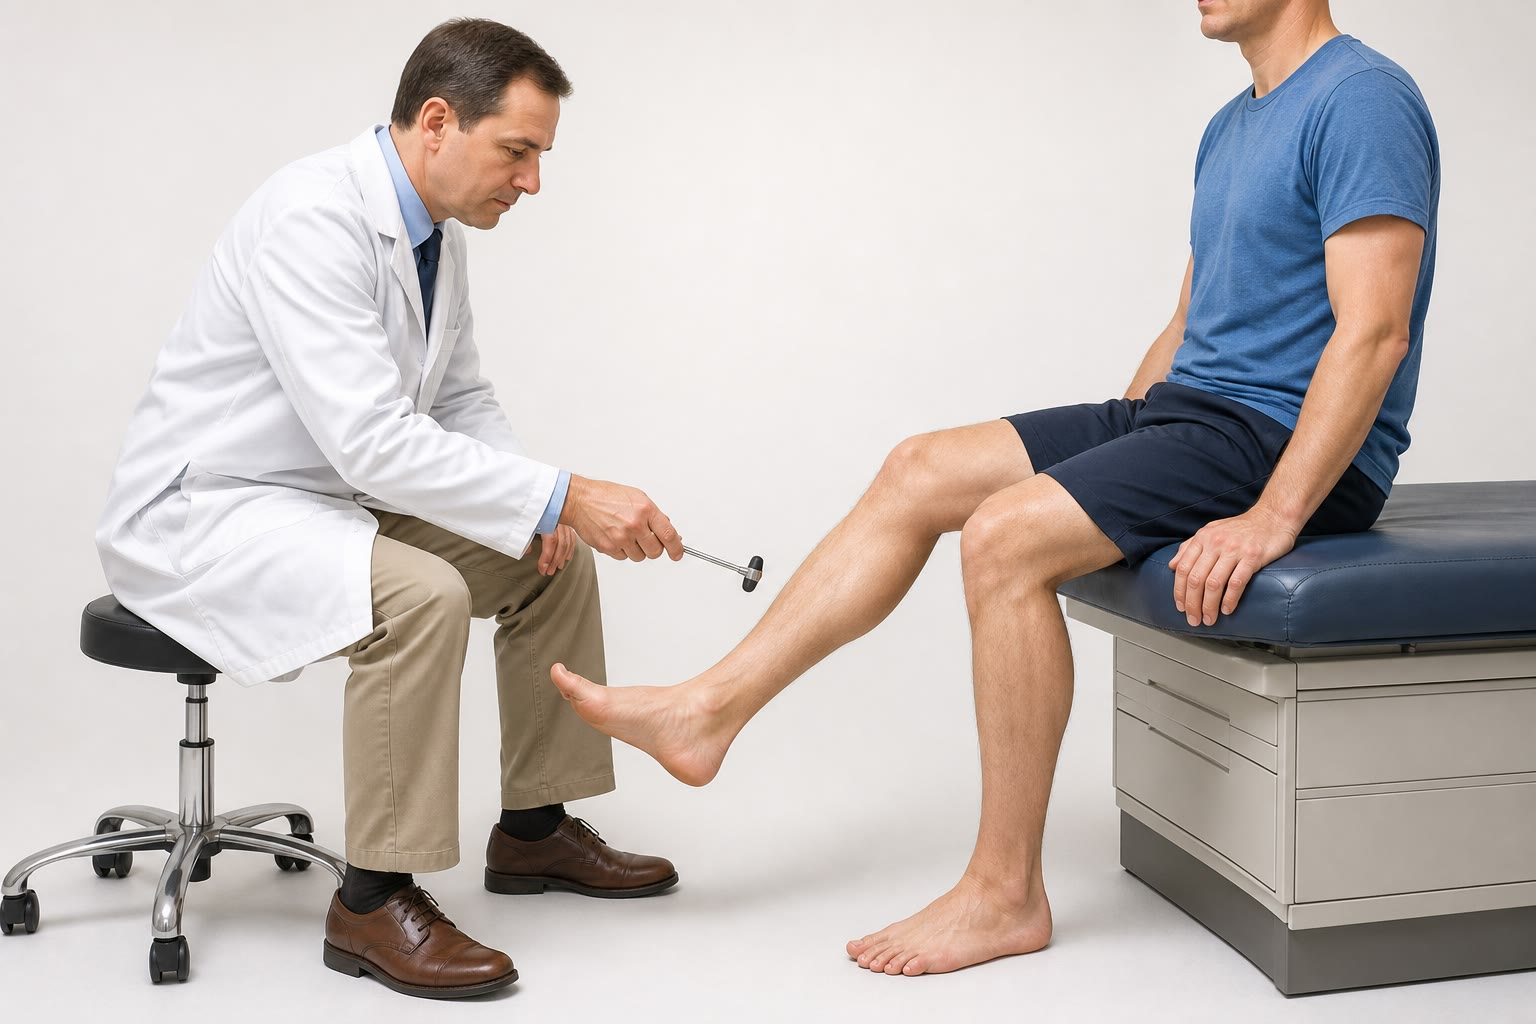
\includegraphics[width=0.56\linewidth]{images/book2/ai/g12-reflex-hammer.jpg}

{\small De knietest: een tik op de kniepees rekt de dijspier uit, en
dertig milliseconden later schopt het been. De \omterm{def:g12:stretch-reflex:reflex}{reflex} controleert in één
seconde de hele boog van spoeltje tot spier.}
\end{omfigure}

\begin{example}[Waar de reflex voor dient]\label{ex:g12:stretch-reflex:posture}
Als je staat, wieg je heen en weer; elke beweging rekt de spieren aan één
kant van de enkel uit, waarvan de spoeltjes vuren en waarvan de
reflexsamentrekking je terugtrekt voordat je het merkt. Als je een blad
draagt, rekt een plotseling extra gewicht de armspieren uit en verstijft
de \omterm{def:g12:stretch-reflex:reflex}{reflex} hen binnen \qty{30}{ms}, voordat het blad kantelt. De \omterm{def:g12:stretch-reflex:reflex}{rekreflex}
is een volgmechanisme: hij verzet zich tegen elke verandering van de
lengte van een spier, en de hersenen stellen zijn gevoeligheid bij om de
spanning van het lichaam te bepalen --- hoger als je je schrap zet, lager
als je slaapt.
\end{example}

\section{Het neuron en zijn boodschap}

\begin{definition}[Neuron]\label{def:g12:stretch-reflex:neuron}
Een \emph{neuron}\index{neuron} is een \omterm{def:g10:cells-common-unit:cell}{cel} die op signaleren is
toegespitst: een cellichaam met zijn kern, vertakte \emph{dendrieten} die
signalen ontvangen, en één enkele lange vezel, het \emph{axon}, dat het
eigen signaal van het neuron naar zijn uiteinden draagt --- bij een
motorisch neuron van het been een meter ver. Vele axonen zijn omwikkeld
met een vettige schede, \emph{myeline}, aangelegd door begeleidende
\omterm{def:g10:cells-common-unit:cell}{cellen}, die het geleiden versnelt. Een zenuw is een bundel van honderden
of duizenden axonen.
\end{definition}

\begin{omfigure}
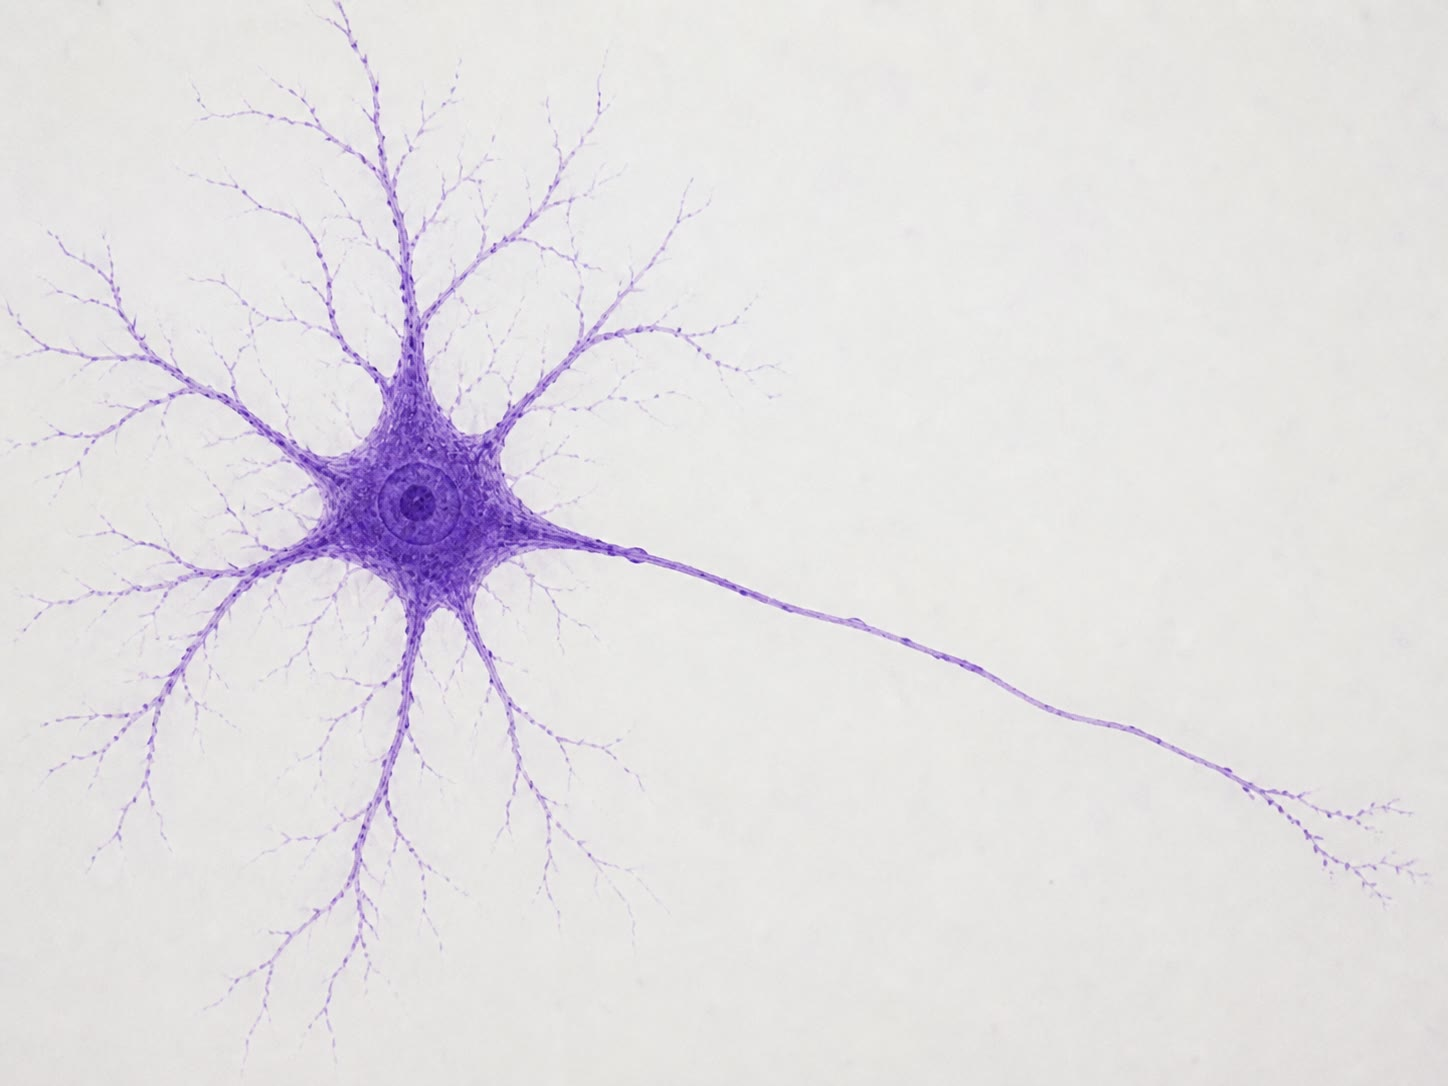
\includegraphics[width=0.5\linewidth]{images/book2/ai/g12-neuron-micrograph.jpg}

{\small Een motorisch \omterm{def:g12:stretch-reflex:neuron}{neuron}, gekleurd: het cellichaam met zijn kern, de
vertakte dendrieten die signalen ontvangen, en het enkele axon dat
vertrekt om de eigen boodschap van het \omterm{def:g12:stretch-reflex:neuron}{neuron} naar een spier te dragen.}
\end{omfigure}

\begin{proposition}[De actiepotentiaal]\label{prop:g12:stretch-reflex:actionpotential}
Het membraan van een \omterm{def:g12:stretch-reflex:neuron}{neuron} houdt een elektrische spanning vast: de
binnenkant staat in rust op ongeveer \qty{-70}{mV} ten opzichte van de
buitenkant. De \emph{zenuwboodschap}\index{zenuwboodschap} is een reeks
\emph{actiepotentialen}\index{actiepotentiaal}: korte omkeringen van die
spanning, die elk tot ongeveer \qty{+30}{mV} stijgen en binnen een
milliseconde terugkeren, en die langs het axon reizen zonder zwakker te
worden. Een \omterm{prop:g12:stretch-reflex:actionpotential}{actiepotentiaal} is \emph{alles of niets}: een prikkel onder
een drempel brengt niets voort, elke prikkel erboven brengt hetzelfde
volledige signaal voort. De sterkte van een prikkel wordt daarom niet in
de grootte van de signalen maar in hun \emph{frequentie} vastgelegd: een
sterkere rek laat het spoeltje meer \omterm{prop:g12:stretch-reflex:actionpotential}{actiepotentialen} per seconde vuren.
\end{proposition}
\begin{proof}[Bewijsmateriaal]
Micro-elektroden die in een axon worden gebracht, nemen de rustspanning op
en, wanneer de \omterm{def:g10:cells-common-unit:cell}{cel} vuurt, gelijke pieken waarvan de vorm niet verandert
met de prikkel of met de afgelegde afstand. Opnames van één spoeltjesvezel
bij toenemende rek tonen pieken van constante grootte met tempo's die van
enkele tot enkele honderden per seconde oplopen. Een prikkel net onder de
drempel geeft helemaal geen piek; een prikkel die al boven de drempel ligt
verdubbelen verandert het tempo, nooit de hoogte.
\end{proof}

\begin{omfigure}
\begin{tikzpicture}
\begin{axis}[
  width=0.62\linewidth, height=5.6cm,
  axis x line=bottom, axis y line=left,
  xmin=0, xmax=5, ymin=-100, ymax=50,
  xlabel={tijd (ms)}, ylabel={membraanspanning (mV)},
  xlabel style={font=\small, at={(axis description cs:0.5,-0.12)}, anchor=north},
  ylabel style={font=\small},
  tick label style={font=\small}, xtick={0,1,2,3,4,5}, ytick={-70,-30,0,30},
  clip=false,
]
\addplot[thick, omThm, smooth] coordinates {(0,-70) (1,-70) (1.3,-55) (1.5,-20) (1.7,30) (1.9,10) (2.1,-40) (2.3,-75) (2.7,-80) (3.2,-72) (4,-70) (5,-70)};
\draw[dashed, gray] (axis cs:0,-55) -- (axis cs:5,-55);
\node[font=\scriptsize, gray, anchor=south west] at (axis cs:3.3,-55) {drempel};
\node[font=\scriptsize, anchor=south west] at (axis cs:0.1,-68) {rust};
\node[font=\scriptsize, anchor=west] at (axis cs:1.8,32) {top};
\end{axis}
\end{tikzpicture}

{\small Een \omterm{prop:g12:stretch-reflex:actionpotential}{actiepotentiaal} opgenomen binnen in een axon: vanaf de
\qty{-70}{mV} van de rust een snelle stijging voorbij de drempel tot
ongeveer \qty{+30}{mV}, een terugkeer tot onder de rustwaarde, en herstel
--- alles in ongeveer twee milliseconden. Elke \omterm{prop:g12:stretch-reflex:actionpotential}{actiepotentiaal} van een
bepaald \omterm{def:g12:stretch-reflex:neuron}{neuron} heeft precies deze vorm.}
\end{omfigure}

\begin{omfigure}
\begin{tikzpicture}[font=\small, line cap=round]
  \foreach \row/\y/\lab/\n in {1/2.4/{zwakke rek}/6, 2/1.2/{matige rek}/12, 3/0/{sterke rek}/24} {
    \draw[thick] (0,\y) -- (9,\y);
    \node[anchor=east] at (-0.2,\y) {\lab};
  }
  \foreach \i in {1,...,6} \draw[very thick, omThm] ({\i*9/7},2.4) -- ({\i*9/7},2.4+0.6);
  \foreach \i in {1,...,12} \draw[very thick, omThm] ({\i*9/13},1.2) -- ({\i*9/13},1.2+0.6);
  \foreach \i in {1,...,24} \draw[very thick, omThm] ({\i*9/25},0) -- ({\i*9/25},0.6);
  \draw[<->] (0,-0.5) -- (9,-0.5) node[midway, below] {\qty{100}{ms}};
\end{tikzpicture}

{\small Vastleggen in frequentie. Dezelfde spoeltjesvezel opgenomen
tijdens drie rekbewegingen: de pieken zijn gelijk, en alleen hun tempo
verandert --- hier ongeveer 60, 120 en 240 per seconde.}
\end{omfigure}

\begin{example}[Snelheid]\label{ex:g12:stretch-reflex:speed}
\omterm{prop:g12:stretch-reflex:actionpotential}{Actiepotentialen} reizen met \qty{1}{m/s} in dunne vezels zonder myeline en
tot \qty{100}{m/s} in de dikke vezels met myeline van de \omterm{def:g12:stretch-reflex:reflex}{rekreflex}. Van de
knie naar het ruggenmerg en terug is ongeveer \qty{1.5}{m}: zo'n
\qty{15}{ms} reizen, waar de reactie van het spoeltje, één \omterm{def:g12:stretch-reflex:synapse}{synaps} en het
op gang brengen van de spier nog eens \qty{15}{ms} bij doen --- de
\qty{30}{ms} van de knieschop. Een boodschap van een teen naar de
hersenen, \qty{1.8}{m} verder, doet er ongeveer \qty{20}{ms} over; de
beslissing om hem te bewegen, en de uitvoering ervan, nog zo'n
\qty{150}{ms}.
\end{example}

\section{De synaps}

\begin{definition}[Synaps en neurotransmitter]\label{def:g12:stretch-reflex:synapse}
Een \emph{synaps}\index{synaps} is de overgang waar het uiteinde van het
axon van het ene \omterm{def:g12:stretch-reflex:neuron}{neuron} de volgende \omterm{def:g10:cells-common-unit:cell}{cel} ontmoet --- een \omterm{def:g12:stretch-reflex:neuron}{neuron} of een
\omterm{def:g10:muscles-and-joints:muscle}{spiervezel} --- over een spleet van zo'n \qty{20}{nm}, de \emph{synaptische
spleet}. Het signaal springt niet elektrisch over de spleet: de
aankomende \omterm{prop:g12:stretch-reflex:actionpotential}{actiepotentialen} laten het uiteinde uit kleine blaasjes een
chemische bode afgeven, de
\emph{neurotransmitter}\index{neurotransmitter}, in de spleet; die bindt
\emph{ontvangers} op het membraan van de ontvangende \omterm{def:g10:cells-common-unit:cell}{cel}, welke de
spanning van die \omterm{def:g10:cells-common-unit:cell}{cel} veranderen; hij wordt daarna binnen enkele
milliseconden vernietigd of teruggenomen. De synaps zet een elektrische
boodschap om in een chemische en weer terug, en de hoeveelheid afgegeven
transmitter --- bepaald door de frequentie van de aankomende
\omterm{prop:g12:stretch-reflex:actionpotential}{actiepotentialen} --- legt de sterkte van de boodschap vast.
\end{definition}

\begin{omfigure}
\begin{tikzpicture}[font=\small, >=Stealth, line cap=round]
  % presynaptic ending
  \draw[thick, fill=omDef!12] (0,0) -- (3.0,0) .. controls (4.0,0) and (4.0,2.6) .. (3.0,2.6) -- (0,2.6);
  \node[anchor=east, align=right, omDef!80!black] at (-0.1,1.3) {uiteinde van het axon\\ (actiepotentialen\\ komen aan)};
  \foreach \x/\y in {2.2/0.7, 2.6/1.3, 2.3/1.9, 1.6/1.2, 3.1/1.0, 3.1/1.7} \draw[thick, fill=omThm!25] (\x,\y) circle (0.22);
  \node[font=\scriptsize, anchor=south] at (1.6,1.5) {blaasjes};
  % cleft
  \draw[thick, fill=omDef!12] (4.6,-0.4) -- (4.6,3.0) -- (8.5,3.0) -- (8.5,-0.4) -- cycle;
  \node[anchor=west, align=left, omMeth!70!black] at (5.0,2.45) {ontvangende cel\\ (neuron of spier)};
  \foreach \y in {0.5,1.1,1.7} \draw[thick, fill=omMeth!40] (4.5,\y-0.15) rectangle (4.85,\y+0.15);
  \node[font=\scriptsize, anchor=west] at (5.0,1.1) {ontvangers};
  % transmitter molecules in cleft
  \foreach \x/\y in {4.05/0.6, 4.25/1.2, 4.1/1.6, 4.3/0.9, 4.2/1.9} \fill[omThm] (\x,\y) circle (2pt);
  \node[font=\scriptsize, anchor=north, align=center] at (4.25,-0.55) {spleet: transmitter\\ afgegeven, dan vernietigd};
  \draw[->, thick] (3.35,1.3) -- (3.95,1.3);
  \draw[->, thick] (4.95,2.1) .. controls (5.6,2.0) .. (6.3,1.5) node[right, font=\scriptsize] {verandering van spanning};
\end{tikzpicture}

{\small Een \omterm{def:g12:stretch-reflex:synapse}{synaps}. \omterm{prop:g12:stretch-reflex:actionpotential}{Actiepotentialen} die het uiteinde bereiken laten
blaasjes de \omterm{def:g12:stretch-reflex:synapse}{neurotransmitter} in de spleet afgeven; die bindt ontvangers op
de ontvangende \omterm{def:g10:cells-common-unit:cell}{cel} en verandert haar spanning; \omterm{def:g11:enzymes-and-phenotype:enzyme}{enzymen} vernietigen hem
daarna. De boodschap steekt over als een chemische stof, en maar in één
richting.}
\end{omfigure}

\begin{proposition}[Prikkeling, remming en de verbinding met de spier]\label{prop:g12:stretch-reflex:junction}
Afhankelijk van de transmitter en zijn ontvanger \emph{prikkelt} een
\omterm{def:g12:stretch-reflex:synapse}{synaps} het ontvangende \omterm{def:g12:stretch-reflex:neuron}{neuron} (brengt het naar zijn drempel toe) of
\emph{remt} zij het (drijft het ervan weg). De \omterm{def:g12:stretch-reflex:reflex}{rekreflex} gebruikt allebei:
prikkeling van het eigen motorische \omterm{def:g12:stretch-reflex:neuron}{neuron} van de spier, remming van dat
van de tegenwerker via het tussenneuron. Bij de \emph{neuromusculaire
verbinding}, de \omterm{def:g12:stretch-reflex:synapse}{synaps} tussen een motorisch \omterm{def:g12:stretch-reflex:neuron}{neuron} en een \omterm{def:g10:muscles-and-joints:muscle}{spiervezel}, is
de transmitter \emph{acetylcholine}: elke \omterm{prop:g12:stretch-reflex:actionpotential}{actiepotentiaal} van het
motorische \omterm{def:g12:stretch-reflex:neuron}{neuron} geeft er genoeg van af om de vezel te laten vuren, en
die trekt samen. Een motorisch \omterm{def:g12:stretch-reflex:neuron}{neuron} en de vezels die het aanstuurt
vormen een \emph{motorische eenheid}; de kracht van een spier wordt
bepaald door hoeveel eenheden vuren en hoe snel.
\end{proposition}
\begin{proof}[Bewijsmateriaal]
Acetylcholine die op een \omterm{def:g10:muscles-and-joints:muscle}{spiervezel} wordt aangebracht laat haar
samentrekken; \emph{curare}, het pijlgif, bindt de acetylcholineontvangers
van de vezel zonder hen te activeren en verlamt elke spier terwijl de
zenuwen blijven vuren; het gif van botulisme blokkeert de afgifte van de
blaasjes en verlamt evenzeer; een insectenbestrijder die het \omterm{def:g11:enzymes-and-phenotype:enzyme}{enzym}
blokkeert dat acetylcholine vernietigt, laat de spieren onbeheersbaar
samentrekken. Strychnine blokkeert de remmende synapsen van het
ruggenmerg, zodat elke rek de samentrekking van zowel de spier als de
tegenwerker uitlokt: stuiptrekkingen. Elk gif noemt een stap van de
verbinding door haar weg te nemen.
\end{proof}

\begin{method}[Een reflex of een gif ontleden]\label{met:g12:stretch-reflex:analyse}
\begin{enumerate}
  \item Volg de boog: ontvanger, sensorisch \omterm{def:g12:stretch-reflex:neuron}{neuron}, centrum, motorisch
        \omterm{def:g12:stretch-reflex:neuron}{neuron}, uitvoerder; bepaal welk onderdeel een letsel of een middel
        raakt.
  \item Vraag je bij elk \omterm{def:g12:stretch-reflex:neuron}{neuron} af wat er wordt vastgelegd --- de
        frequentie van de \omterm{prop:g12:stretch-reflex:actionpotential}{actiepotentialen} --- en bij elke \omterm{def:g12:stretch-reflex:synapse}{synaps} wat de
        boodschap draagt --- de transmitter en zijn hoeveelheid.
  \item Zoek bij een gif de stap die het raakt: de afgifte van de
        transmitter, de ontvanger, de vernietiging van de transmitter, of
        een remmende \omterm{def:g12:stretch-reflex:synapse}{synaps}; voorspel verlamming (er komt niets door) of
        stuiptrekking (er wordt niets tegengehouden).
  \item Reken de tijd uit: afstand gedeeld door de geleidingssnelheid,
        plus ongeveer een milliseconde per \omterm{def:g12:stretch-reflex:synapse}{synaps}.
\end{enumerate}
\end{method}

\begin{remark}[Een boodschap gemaakt van dezelfde pieken]\label{rem:g12:stretch-reflex:spikes}
Elke boodschap in het zenuwstelsel --- de rek van het spoeltje, het licht
van het netvlies, het bevel van de hersenen om te bewegen --- bestaat uit
dezelfde alles-of-niets-actiepotentialen, die alleen in tempo verschillen
en in de draden die hen dragen; de betekenis ligt in welk \omterm{def:g12:stretch-reflex:neuron}{neuron} vuurt,
niet in wat het vuurt. En bij elke \omterm{def:g12:stretch-reflex:synapse}{synaps} wordt de boodschap een dosis van
een chemische stof, en daarom kan een molecule --- een transmitter, een
gif, een medicijn --- op elk punt aan het gesprek deelnemen. Het laatste
hoofdstuk volgt dezelfde pieken en synapsen omhoog tot in de hersenen, en
het bevel dat weer omlaag komt.
\end{remark}

\section{Oefeningen}

\begin{exercise}[$\star$]\label{exo:g12:stretch-reflex:1}
Noem de vijf onderdelen van de boog van de \omterm{def:g12:stretch-reflex:reflex}{rekreflex}, op volgorde.
\end{exercise}

\begin{exercise}[$\star$]\label{exo:g12:stretch-reflex:2}
Beschrijf de delen van een \omterm{def:g12:stretch-reflex:neuron}{neuron} en de richting waarin zijn boodschap
reist.
\end{exercise}

\begin{exercise}[$\star$]\label{exo:g12:stretch-reflex:3}
Wat is een \omterm{prop:g12:stretch-reflex:actionpotential}{actiepotentiaal}? Wat betekent "alles of niets", en hoe wordt de
sterkte vastgelegd?
\end{exercise}

\begin{exercise}[$\star$]\label{exo:g12:stretch-reflex:4}
Beschrijf wat er bij een \omterm{def:g12:stretch-reflex:synapse}{synaps} gebeurt, van de aankomst van de
\omterm{prop:g12:stretch-reflex:actionpotential}{actiepotentialen} tot de reactie van de ontvangende \omterm{def:g10:cells-common-unit:cell}{cel}.
\end{exercise}

\begin{exercise}[$\star$]\label{exo:g12:stretch-reflex:5}
Welke transmitter werkt bij de neuromusculaire verbinding, en wat doen
curare en het botulinegif er elk mee?
\end{exercise}

\begin{exercise}[$\star\star$]\label{exo:g12:stretch-reflex:6}
Tel in de figuur over het vastleggen in frequentie de pieken in
\qty{100}{ms} voor elke rek en geef de tempo's. Wat verandert er niet
tussen de rijen?
\end{exercise}

\begin{exercise}[$\star\star$]\label{exo:g12:stretch-reflex:7}
De vertraging van de knieschop is \qty{30}{ms} over een weg van
\qty{1.5}{m}. Bereken de geleidingssnelheid van de vezels als de \omterm{def:g12:stretch-reflex:synapse}{synaps} en
het op gang brengen van de spier samen \qty{12}{ms} kosten.
\end{exercise}

\begin{exercise}[$\star\star$]\label{exo:g12:stretch-reflex:8}
Leg uit waarom de achterwortel doorsnijden de \omterm{def:g12:stretch-reflex:reflex}{reflex} opheft maar niet het
vermogen van de spier om samen te trekken, en waarom de voorwortel
doorsnijden allebei opheft.
\end{exercise}

\begin{exercise}[$\star\star$]\label{exo:g12:stretch-reflex:9}
Waarom moet de tegenwerkende spier tijdens de \omterm{def:g12:stretch-reflex:reflex}{reflex} worden geremd? Welk
onderdeel van de boog doet dat, en via wat voor type \omterm{def:g12:stretch-reflex:synapse}{synaps}?
\end{exercise}

\begin{exercise}[$\star\star$]\label{exo:g12:stretch-reflex:10}
Een prikkel van 2 eenheden ligt precies op de drempel van een \omterm{def:g12:stretch-reflex:neuron}{neuron} en
geeft één \omterm{prop:g12:stretch-reflex:actionpotential}{actiepotentiaal} van \qty{100}{mV}. Voorspel het signaal bij
prikkels van 1, 4 en 8 eenheden.
\end{exercise}

\begin{exercise}[$\star\star$]\label{exo:g12:stretch-reflex:11}
Leg uit waarom de boodschap een \omterm{def:g12:stretch-reflex:synapse}{synaps} maar in één richting oversteekt, en
waarom zij daar ongeveer een milliseconde wordt opgehouden.
\end{exercise}

\begin{exercise}[$\star\star\star$]\label{exo:g12:stretch-reflex:12}
Een insectenbestrijder blokkeert het \omterm{def:g11:enzymes-and-phenotype:enzyme}{enzym} dat acetylcholine vernietigt.
Voorspel zijn gevolg bij de neuromusculaire verbinding en voor de
ademhaling, en leg uit waarom een middel dat de acetylcholineontvangers
blokkeert in een zorgvuldig afgemeten dosis als tegengif wordt gebruikt.
\end{exercise}

\begin{exercise}[$\star\star\star$]\label{exo:g12:stretch-reflex:13}
Strychnine blokkeert remmende synapsen in het ruggenmerg. Leg met de
\omterm{def:g12:stretch-reflex:reflex}{reflexboog} uit waarom een lichte aanraking dan stuiptrekkingen van het
hele lichaam uitlokt.
\end{exercise}

\begin{exercise}[$\star\star\star$]\label{exo:g12:stretch-reflex:14}
Bij iemand met beschadigd myeline is de vertraging van de knieschop
\qty{60}{ms} in plaats van 30. Bereken de geleidingssnelheid die daaruit
volgt (met de getallen van oefening 7) en leg uit waarom myeline uitmaakt.
\end{exercise}

\begin{exercise}[$\star\star\star$]\label{exo:g12:stretch-reflex:15}
"Het ruggenmerg is alleen maar een kabel tussen de hersenen en het
lichaam." Herschrijf dit in een alinea zoals het hoort, met de \omterm{def:g12:stretch-reflex:reflex}{reflex}, het
tussenneuron, en het dier waarvan het merg van zijn hersenen is
afgesneden.
\end{exercise}

\section{Probleem: Dertig milliseconden}

\begin{problem}[{Weekendprobleem --- de knieschop op de klok gelegd en uit
elkaar gehaald: de code van het spoeltje, de snelheid van de vezels, de
vertraging van de synaps, de scheikunde van de verbinding, en de giffen
die elke stap benoemen}]
\label{pb:g12:stretch-reflex:1}
Elektroden nemen de elektrische activiteit van de dijspier van een
proefpersoon op (een elektromyogram) terwijl er op de kniepees wordt
getikt. Het signaal van de spier begint \qty{30}{ms} na de tik; het been
beweegt \qty{20}{ms} later. De afstand van de \omterm{def:g10:muscles-and-joints:muscle}{pees} tot het ruggenmerg
langs de zenuw is \qty{75}{cm}, en evenveel terug.

\medskip
\noindent\textbf{Deel I --- Het tijdsverloop.}
\begin{enumerate}
  \item Bereken de totale lengte van de zenuwweg van de \omterm{def:g12:stretch-reflex:reflex}{reflex}.
  \item Neem aan dat de reactie van het spoeltje en het op gang brengen
        van de spier elk \qty{4}{ms} vergen, en de \omterm{def:g12:stretch-reflex:synapse}{synaps} \qty{1}{ms}.
        Hoeveel van de \qty{30}{ms} is geleiding, en wat is de
        geleidingssnelheid?
  \item Voorspel de vertraging bij een proefpersoon die \qty{20}{cm} langer
        is, met dezelfde vezels.
  \item Waarom beweegt het been \qty{20}{ms} nadat het elektrische signaal
        van de spier begint?
  \item Er wordt een proefpersoon gezegd de tik te verwachten en "eraan te
        denken" de schop tegen te houden; de schop verandert niet. Verklaar
        dat met het tijdsverloop van een boodschap naar en van de hersenen
        (\qty{1.2}{m} vezel extra, en verscheidene synapsen).
\end{enumerate}

\medskip
\noindent\textbf{Deel II --- De code.}
De vezel van het spoeltje vuurt in rust 20 \omterm{prop:g12:stretch-reflex:actionpotential}{actiepotentialen} per seconde,
tijdens de tik 200.
\begin{enumerate}[resume]
  \item Hoeveel \omterm{prop:g12:stretch-reflex:actionpotential}{actiepotentialen} stuurt het spoeltje in de \qty{10}{ms} na
        de tik? Wat verandert er tussen rust en tik, en wat niet?
  \item Elke \omterm{prop:g12:stretch-reflex:actionpotential}{actiepotentiaal} die bij de \omterm{def:g12:stretch-reflex:synapse}{synaps} aankomt geeft een vaste
        hoeveelheid transmitter af. Met welke factor stijgt de per seconde
        afgegeven transmitter tijdens de tik?
  \item Het motorische \omterm{def:g12:stretch-reflex:neuron}{neuron} vuurt alleen als er binnen enkele
        milliseconden genoeg transmitter aankomt. Leg uit waarom het tempo
        in rust de spier niet laat samentrekken, en het tempo bij de tik
        wel.
  \item Een zachtere tik geeft er 100 per seconde. Voorspel de reactie van
        het motorische \omterm{def:g12:stretch-reflex:neuron}{neuron} en de kracht van de schop, met de motorische
        eenheden.
  \item Leg uit waarom de boodschap van een spoeltje niet in de grootte van
        zijn \omterm{prop:g12:stretch-reflex:actionpotential}{actiepotentialen} zou kunnen worden vastgelegd.
\end{enumerate}

\medskip
\noindent\textbf{Deel III --- De verbinding.}
\begin{enumerate}[resume]
  \item Noem de transmitter bij de neuromusculaire verbinding en beschrijf
        wat er na zijn werking met hem gebeurt.
  \item Er wordt curare ingespoten: het elektromyogram toont na de tik geen
        signaal, maar de zenuw draagt nog altijd \omterm{prop:g12:stretch-reflex:actionpotential}{actiepotentialen}. Welke
        stap is geblokkeerd?
  \item In plaats daarvan botulinegif: hetzelfde elektromyogram, hetzelfde
        zenuwsignaal. Welke stap, en hoe zou je de twee in het laboratorium
        uit elkaar houden?
  \item Een verdovingsmiddel blokkeert de \omterm{prop:g12:stretch-reflex:actionpotential}{actiepotentialen} in de
        sensorische vezels. Welke opnames verdwijnen, en welke blijven?
  \item Leg uit waarom alle drie een slap been opleveren maar langs drie
        verschillende mechanismen.
\end{enumerate}

\medskip
\noindent\textbf{Deel IV --- Het centrum.}
\begin{enumerate}[resume]
  \item Tijdens de schop is het elektromyogram van de kniebuigers stil, en
        zakt het onder zijn rustwaarde. Verklaar dat met het tussenneuron.
  \item Een patiënt van wie het ruggenmerg boven de hoogte van de \omterm{def:g12:stretch-reflex:reflex}{reflex} is
        doorgesneden, heeft nog altijd een knieschop --- en een overdreven
        sterke. Wat laat het bestaan van de \omterm{def:g12:stretch-reflex:reflex}{reflex} zien, en wat doet zijn
        overdrevenheid vermoeden over de gewone rol van de hersenen?
  \item Noem bij een patiënt bij wie de \omterm{def:g12:stretch-reflex:reflex}{reflex} aan één kant ontbreekt de
        onderdelen van de boog die beschadigd zouden kunnen zijn, en één
        test om de schade te lokaliseren.
  \item Waarom toetsen artsen deze \omterm{def:g12:stretch-reflex:reflex}{reflex} standaard, in enkele seconden,
        bij elke patiënt?
  \item Geef het resultaat: de geleidingssnelheid van de vezels van de
        \omterm{def:g12:stretch-reflex:reflex}{reflex}, de grootheid die de sterkte van de rek vastlegt, en de ene
        chemische stap waar curare op werkt.
\end{enumerate}
\end{problem}
